\section{Features}
\greenbf{Desirable properties:} shift, rotation, scale, brightness invariant
\subsection*{Edge Detection}
How to tell if there is an edge? Local maxima of the first derivative and the zero crossing of the second derivative.\\
\greenbf{Edge detection filters:}

\greenbf{Sobel:}\\
$K_x = \begin{bmatrix}
    %\begin{smallmatrix}
        -1 & 0 & 1\\
        -2 & 0 & 2\\
        -1 & 0 & 1
    %\end{smallmatrix}
\end{bmatrix}$,
$K_y = \begin{bmatrix}
    %\begin{smallmatrix}
        -1 & -2 & -1\\
        0 & 0 & 0\\
        1 & 2 & 1
    %\end{smallmatrix}
\end{bmatrix}$

\greenbf{Prewitt:}\\
$K_x = \begin{bmatrix}
    %\begin{smallmatrix}
        -1 & 0 & 1\\
        -1 & 0 & 1\\
        -1 & 0 & 1
    %\end{smallmatrix}
\end{bmatrix}$,
$K_y = \begin{bmatrix}
    %\begin{smallmatrix}
        -1 & -1 & -1\\
        0 & 0 & 0\\
        1 & 1 & 1
    %\end{smallmatrix}
\end{bmatrix}$

\greenbf{Roberts:}\\
$K_x = \begin{bmatrix}
    %\begin{smallmatrix}
        1 & 0\\
        0 & -1
    %\end{smallmatrix}
\end{bmatrix}$,
$K_y = \begin{bmatrix}
    %\begin{smallmatrix}
        0 & 1\\
        -1 & 0
    %\end{smallmatrix}
\end{bmatrix}$

\greenbf{Gradient Magnitude:}\\
$M(x, y) = \sqrt{(\frac{\partial f}{\partial x})^{2} + (\frac{\partial f}{\partial y})^{2}}$\\
\greenbf{Gradient Angle:} \\
$\alpha(x, y) = \tan^{-1}(\frac{\partial f}{\partial y} / \frac{\partial f}{\partial x})$
\subsection*{Laplacian operator}
detect discontinuities by considering second derivative
$\begin{bmatrix}
    %\begin{smallmatrix}
        0 & 1 & 0\\
        1 & -4 & 1\\
        0 & 1 & 0
    %\end{smallmatrix}
\end{bmatrix}
\quad \text{or} \quad
\begin{bmatrix}
    %\begin{smallmatrix}
        1 & 1 & 1\\
        1 & -8 & 1\\
        1 & 1 & 1
    %\end{smallmatrix}
\end{bmatrix}$
are discrete space approximations. Is isotropic\graytext{(rotationally invariant)}, zero crossings make edge locations. Sensitive to fine details and noise \graytext{($\rightarrow$ smoothing before applying)}.\\ blur image first \graytext{(LoG)}\\
\greenbf{Laplacian of Gaussian \graytext{(LoG)}:} convolve gaussian blurring and laplacian operator in LoG operator \graytext{(cheaper)} $LoG(x, y) = -\frac{1}{\pi \sigma^{4}} (1 - \frac{x^{2} + y^{2}}{2\sigma^{2}}) e^{-\frac{x^{2} + y^{2}}{2\sigma^{2}}}$
\subsection*{Canny Edge Detector: 5 Steps}
\begin{compactenum}
    \item smooth image with a Gaussian filter
    \item compute gradient magnitude and angle using Sobel/Prewitt/...
    \item apply non-maximum suppression to gradient magnitude image \graytext{(Quantize edge normal to one of four directions: horizontal, +45°, vertical, -45°. If $M(x, y))$ smaller than either of its neighbors in edge normal direction suppress, else keep}
    \item Double thresholding for intensity to detect strong and weak edge pixels
    \item Reject weak edge pixels not connected to strong edge pixels
\end{compactenum}
\subsection*{Hough Transform}
Fitting a straight line to a set of edge pixels\\
\includegraphics*[width = \columnwidth]{jo/slope.png}\\
\greenbf{Alternative parameterization:}\\
$x \cos(\theta) + y \sin(\theta) = \rho$ \\
$(x - a)^{2} + (y - a)^{2} = r^{2}$
\greenbf{For circles:} if r known: calculate circles with radius r around edge pixels $\rightarrow$ intersection (local maxima) of circles gives center.\\ Where lots of them meet is the center of a circle. else: use 3D hough transform with parameters $(x_0, y_0, r)$
Each point $(x_i, y_i)$ in the $xy$-plane gives a sinusoid in the $\theta \rho$ plane. Colinear points lying on the line give curves intersecting at the same point in the polar parameter plane. Local maxima give significant lines.
\subsection*{Corner Detection}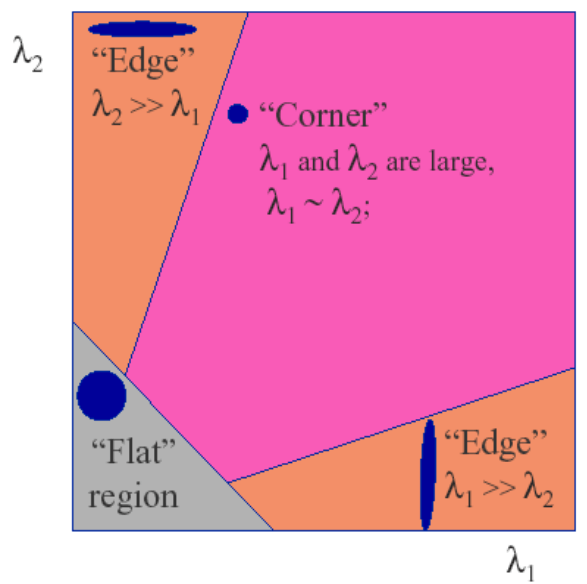
\includegraphics[width = 2cm]{jo/corner.png}\\
Edges are only well localized in one direction $\rightarrow$ detect corners.\\
Desirable properties: Acute localization, invariance against shift, rotation, scale, brightness change, robust against noise, high repeatability\\
\greenbf{Linear approximation for small $\Delta x \Delta y$:} (Taylor) $f(x + \Delta x, y + \Delta y) \approx f(x, y) + f_x(x, y) \Delta x + f_y(x, y)\Delta y$
\subsection*{Local displacement sensitivity \graytext{(Harris corners)}}
$S (\Delta x, \Delta y) = (\Delta x \Delta y) \left( \sum_{x, y \in \text{window}}
\begin{bmatrix}
    \begin{smallmatrix} 
        f_x^{2} & f_x f_y \\ 
        f_x f_y & f_y^{2} 
    \end{smallmatrix} 
\end{bmatrix}
\right)
\begin{bmatrix}
    \begin{smallmatrix} 
        \Delta x \\ 
        \Delta y
    \end{smallmatrix} 
\end{bmatrix}  \\
\approx \text{SSD}$.
Find points where $\min \Delta^T M \Delta$ is large for $||\Delta || = 1$ i. e. maximize the eigenvalues of $M$\\
\greenbf{Harris cornerness:} Measure of cornerness\\
$C(c, y) = \det(M) - k * trace(M)^{2} = \lambda_1\lambda_2 + k(\lambda_1 + \lambda_2)$ \\
\greenbf{Robustness of Harris corner detector:} Invariant to brightness offset, invariant to shift and rotation but not to scaling!
$\lambda_1 >> \lambda_2 \rightarrow$ edge, $\lambda_1$ and $ \lambda_2$ large $\rightarrow$ corner, else $\rightarrow$ flat region.\\
not scale invariant: \includegraphics*[width = 4cm]{jo/corner-edge.png}\\
\greenbf{Overcome issues:} look for strong DoG response or consider local maxima in position and scale space, Gaussian weighing.
\subsection*{Lowe's SIFT features}
Look for strong responses of difference of Gaussians \graytext{(DoG)} filter, only look at local maxima in both position and scale.\\
\greenbf{DoG:} $DoG(x, y) = \frac{1}{k}* e^{-\frac{x^{2} + y^{2}}{(k\sigma)^{2}}} - e^{-\frac{x^{2} + y^{2}}{\sigma^{2}}}$ e.g. $k = \sqrt{2}$\\
Orientation: create histogram of local gradient directions computed at selected scale, assign canonical orientation at peak of smoothed histogram. Get a SIFT descriptor \graytext{(threshold image gradients are sampled over $16\times 16$ array of locations in scale space)} and do matching with these. Invariant to scale, rotation, illumination and viewpoint.
\greenbf{Limits local gradient}
\begin{compactenum}
    \item fails when intensity structure within window is poor
    \item fails when displacement is large (typical operating range is motion of 1 pixel per iteration!)
    \item also brightness is not strictly constant in images
\end{compactenum}
\textbf{Solution:} Pyramid, coarse to fine
